\section{Getting Started (Day 1)}

\myCenteredBox[width=5in,colback=white,sharp corners,]{
    Today you will 
    \begin{itemize}[nosep,label=\checkmark]
        \item break into teams,
        \item build catapults,
        \item test them with \mymm{}s, and 
        \item practice taking measurements.
    \end{itemize}
}


\subsection{Teams}

You may work in groups of up to 4 people. Or you may work on your own.
There are four ``roles''. If you have several people on your team, 
each person must have a role. Record that information here.

\myCenteredBox[colback=\myFillinColor]{
    \centering
    \renewcommand{\arraystretch}{1.5}
    \begin{tabular}{l|p{3in}|p{3in}}
        \toprule
        {\itshape role} & {\itshape what?} & {\itshape who?} \\
        \toprule
        {\bfseries\itshape launcher} & hold and launch the catapult. & \\
        \midrule
        {\bfseries\itshape timer}    & time the flight of the \mymm{}s&\\
        \midrule
        {\bfseries\itshape measurer} & measure how far the \mymm~flew&\\
        \midrule
        {\bfseries\itshape recorder} & write down all the times and measurements&\\
        \bottomrule
    \end{tabular}
}

\subsection{Catapult Construction}

Each team will build a catapult from tongue depressor sticks and rubber bands.
Here are the steps.
Check them off when you have completed them.
\myCenteredBox[colback=\myFillinColor]{
    \begin{itemize}[label={\Large$\Box$}]
        \item Wind a rubber band several times around one end of a stick 
            so that the rubber band stays in place.
            Your \mymm{}s will rest against this rubber band when you launch.
        \item Put a second stick next to the first one. Wrap a rubber band around the other end of them
            to hold them tightly together. 
        \item Insert a pencil between the two sticks. 
            You might want to use more rubber bands so that the pencil 
            does not easily move back and forth.
            The gap created by the pencil is what makes the catapult ``spring''.
    \end{itemize}
}

If you do not understand these instructions, look at the catapults of other teams, or come look at mine.
If you do not understand how the catapult works, ask me to show you.

Give your catapult a {name}.
\myCenteredBox[colback=\myFillinColor]{
    \centering
    {\itshape name:} \fbox{\phantom{\LARGE Xxxxxx Xxxxxx-Xxxxxx}}
}

\subsection{Dry Runs}

Now it is time to try out your catapult. 
Find a clear space, and try launching an \mymm. 
This will give you a feel for how it works and how much space you need.

Here is the general idea.
\begin{itemize}[nosep]
    \item You will launch your \mymm{}s from your catapult.
    \item The candy will fly across the room following a parabolic trajectory.
    \item The candy will {\scshape Land} at a point ``downrange'' of the {\scshape Launch} point.
    \item You will measure the downrange distance.
    \item You will time how long the candy is in the air (from launch to landing).
\end{itemize}

\begin{center}
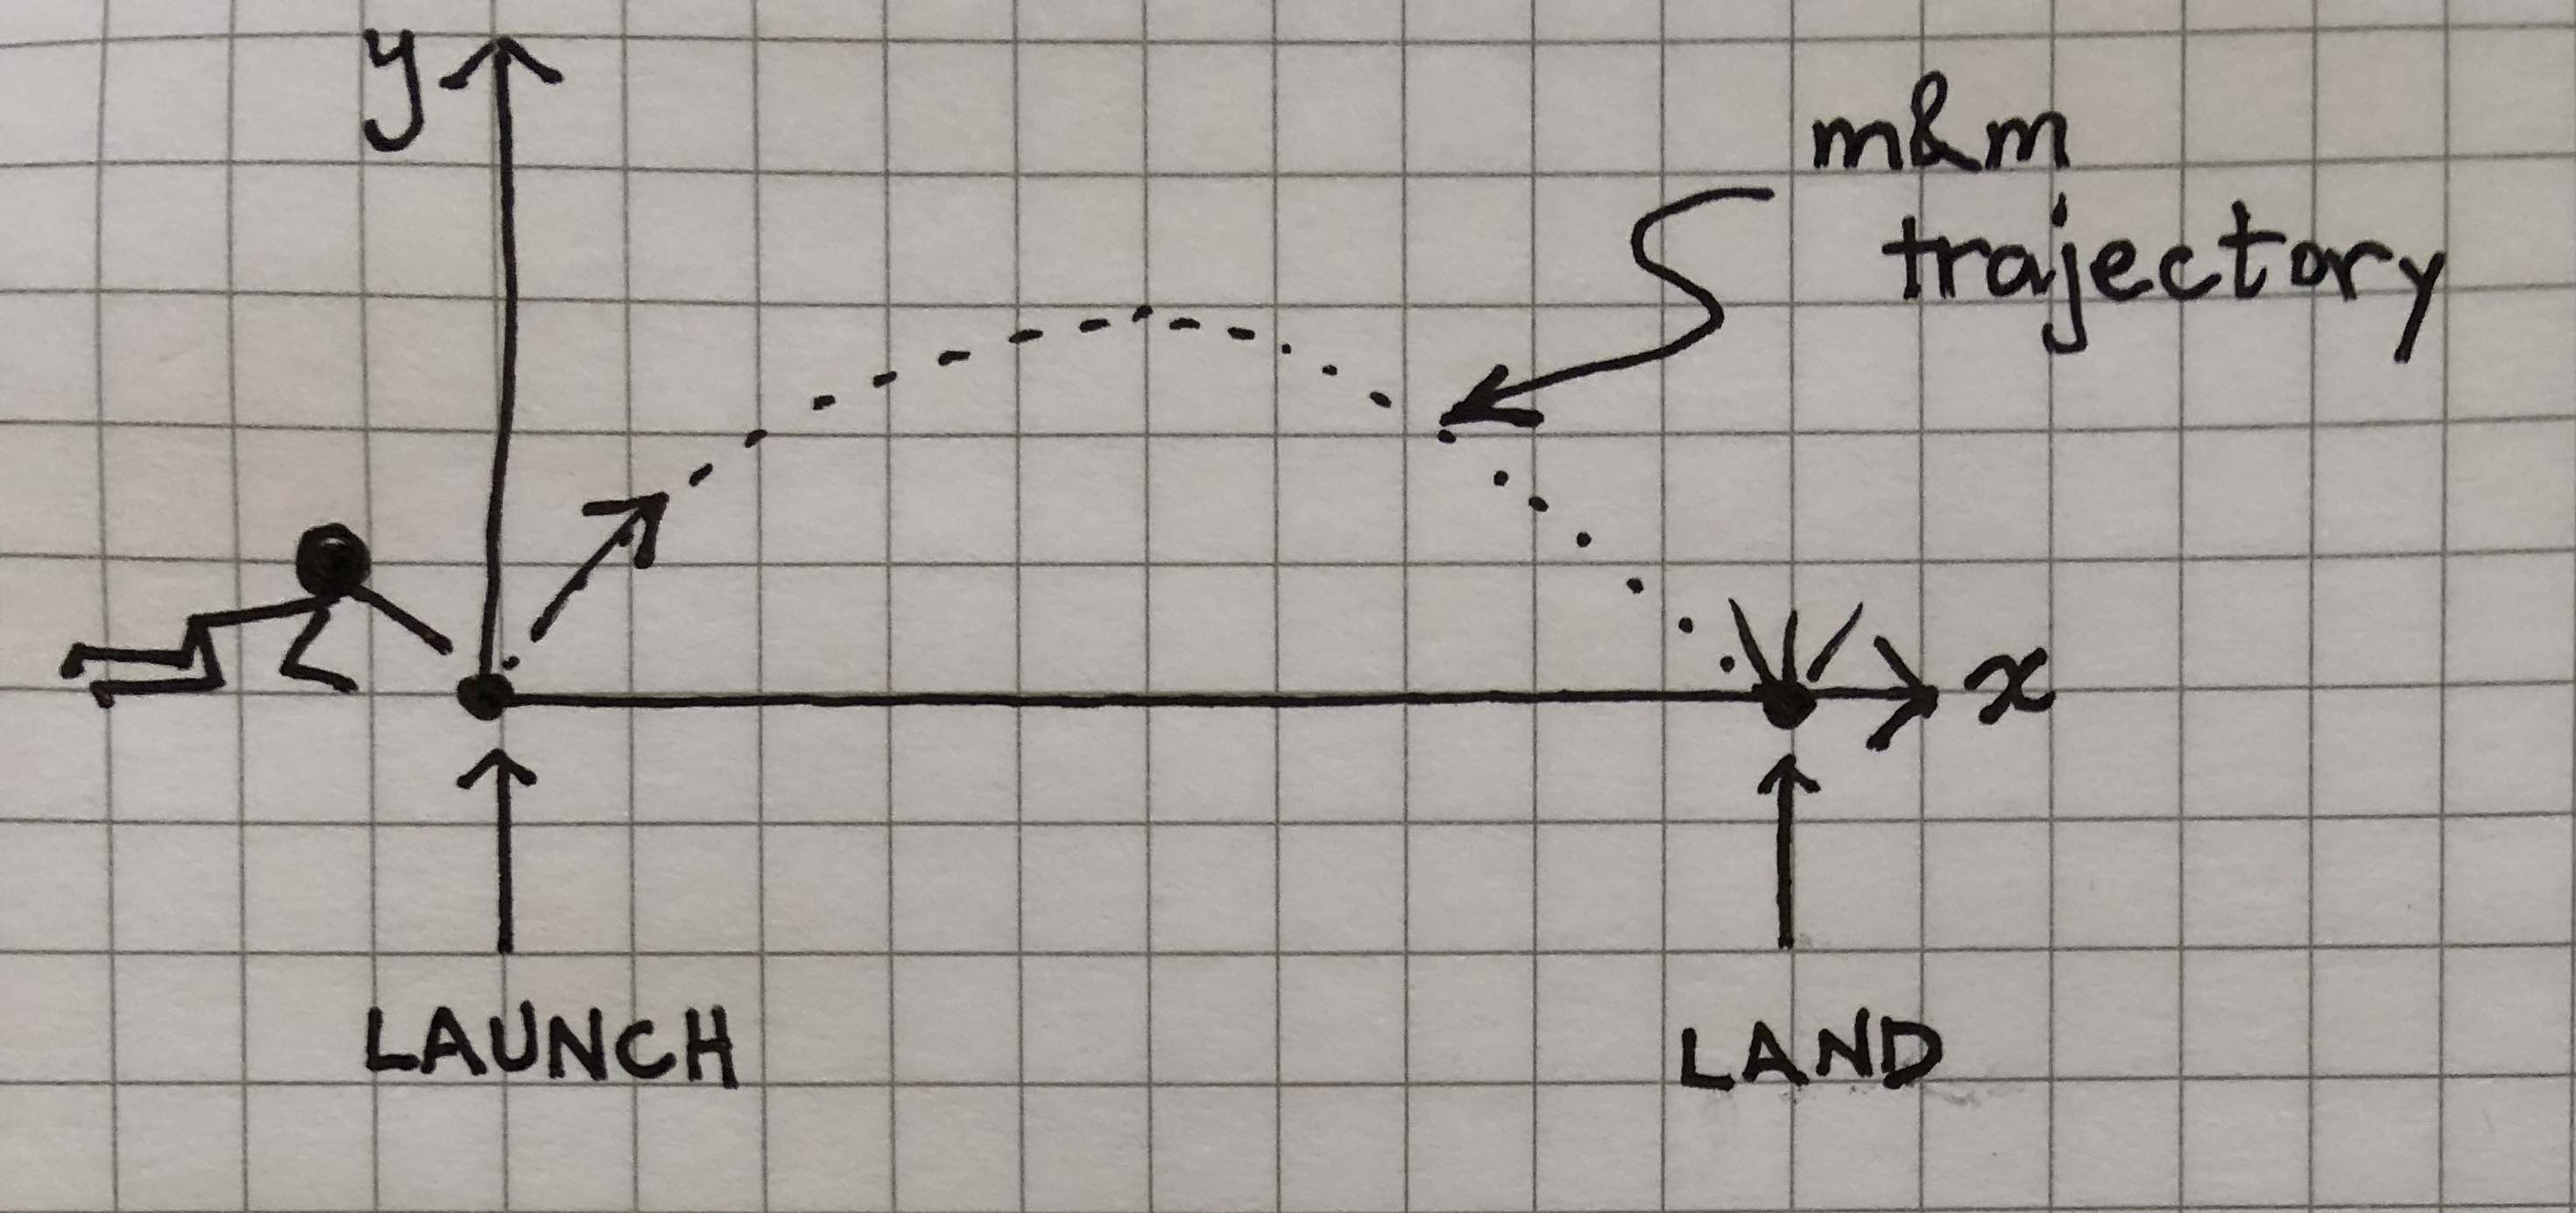
\includegraphics[width=3in]{../launch-and-landing.jpg}
\end{center}

Practice timing and measuring the flight of your \mymm{}s. 
Launch {\bfseries\itshape at least 3} \mymm{}s. 
\begin{itemize}[nosep]
    \item The {\bfseries\itshape timer} person should use their phone to determine 
        the {\bfseries\itshape flight time} (in seconds) of each test trajectory.
    \item The {\bfseries\itshape measurer} should use a yardstick to measure 
        the {\bfseries\itshape downrange distance} (in centimeters) of each test trajectory.
    \item The {\bfseries\itshape recorder} should write those values down.
    \item Everyone should copy those values into their packets below.
\end{itemize}

\myCenteredBox[colback=\myFillinColor]{
    \centering
    \renewcommand{\arraystretch}{1.5}
    \begin{tabular}{c|p{2in}|p{2in}}
        \toprule
        {\itshape dry run \#} & {\itshape fight time (sec)} & {\itshape downrange distance (cm)} \\
        \toprule
        1 & & \\
        \midrule
        2 & & \\
        \midrule
        3 & & \\
        \bottomrule
    \end{tabular}
}

Are your times and distances all approximately the same? 
\myCenteredBox[colback=\myFillinColor]{
    \centering 
    \qquad
    {\scshape Yes}
    \qquad
    {\scshape No}
    \qquad
    (circle one)
}

If not, write a short explanation of what was different and 
what you think explains the difference.%
\footnote{%
    For example:%
    ``The second dry run was messed up since we didn't 
    start timing right when the catapault launched.''
}

\myCenteredBox[colback=\myFillinColor]{
    \vspace{1em}
    \underline{\hspace{\textwidth}}\\[0.5\baselineskip]
    \underline{\hspace{\textwidth}}\\[0.5\baselineskip]
    \underline{\hspace{\textwidth}}\\[0.5\baselineskip]
    \underline{\hspace{\textwidth}}\\[0.5\baselineskip]
    \underline{\hspace{\textwidth}}\\[0.5\baselineskip]
    \underline{\hspace{\textwidth}}\\
}
